\subsection{Testbenches}

Some testbenches have been written for the biggest modules of the project. The only notable exception is the 
controller for time but also since it is mostly tested by the general CPU testbench. So here is the testbench that has been written:

\begin{enumerate}[label={\textbullet}]
    \item ALU
    \item Branch Unit
    \item CPU
    \item Forward controller
    \item LSU
    \item PC
    \item Register File
    \item Stall Unit
\end{enumerate}

Most of this testbench is testing the module with a lot of different (mostly random) inputs and checking that the output is correct.
Some are also testing more specific cases like corner cases that could lead to some issues in the design. The testbench for the CPU is 
a bit special since it is testing the whole CPU with a simple program computing a recursive sum of the first 10 integers testing most 
of the module of the CPU.
When writing the test I discovered some issues in the design, mostly in the ALU and the Branch Unit. For in the ALU I was shifting 
not correctly in one of my instructions, and in the Branch Unit the output of the alu wasn't treated as a signed number.
It's also with the CPU testbench that I've discovered the issue with the different values between Questa Modelsim with full visibility and 
Icarus Verilog. 
I still think that more tests could be added to the different testbenches to have even better coverage like for example for the CPU with a 
program that could use every single instruction of the CPU. But I think that the current state is pretty okay. \\

The process of actually launching the test and seeing the output has been simplified by me by creating a Makefile that will compile all the 
different modules correctly and link them together and it will launch the simulation and output the results into the terminal. Also, each 
testbench will generate a .vcd file that can be opened with GTKWave to see the different signals of the simulation. It is important to have
Icarus Verilog for that part to work since it doesn't use any containers that could improve portability but I think it's not needed 
in my opinion but that could be a nice improvement.

\begin{figure}[H]
    \centering
    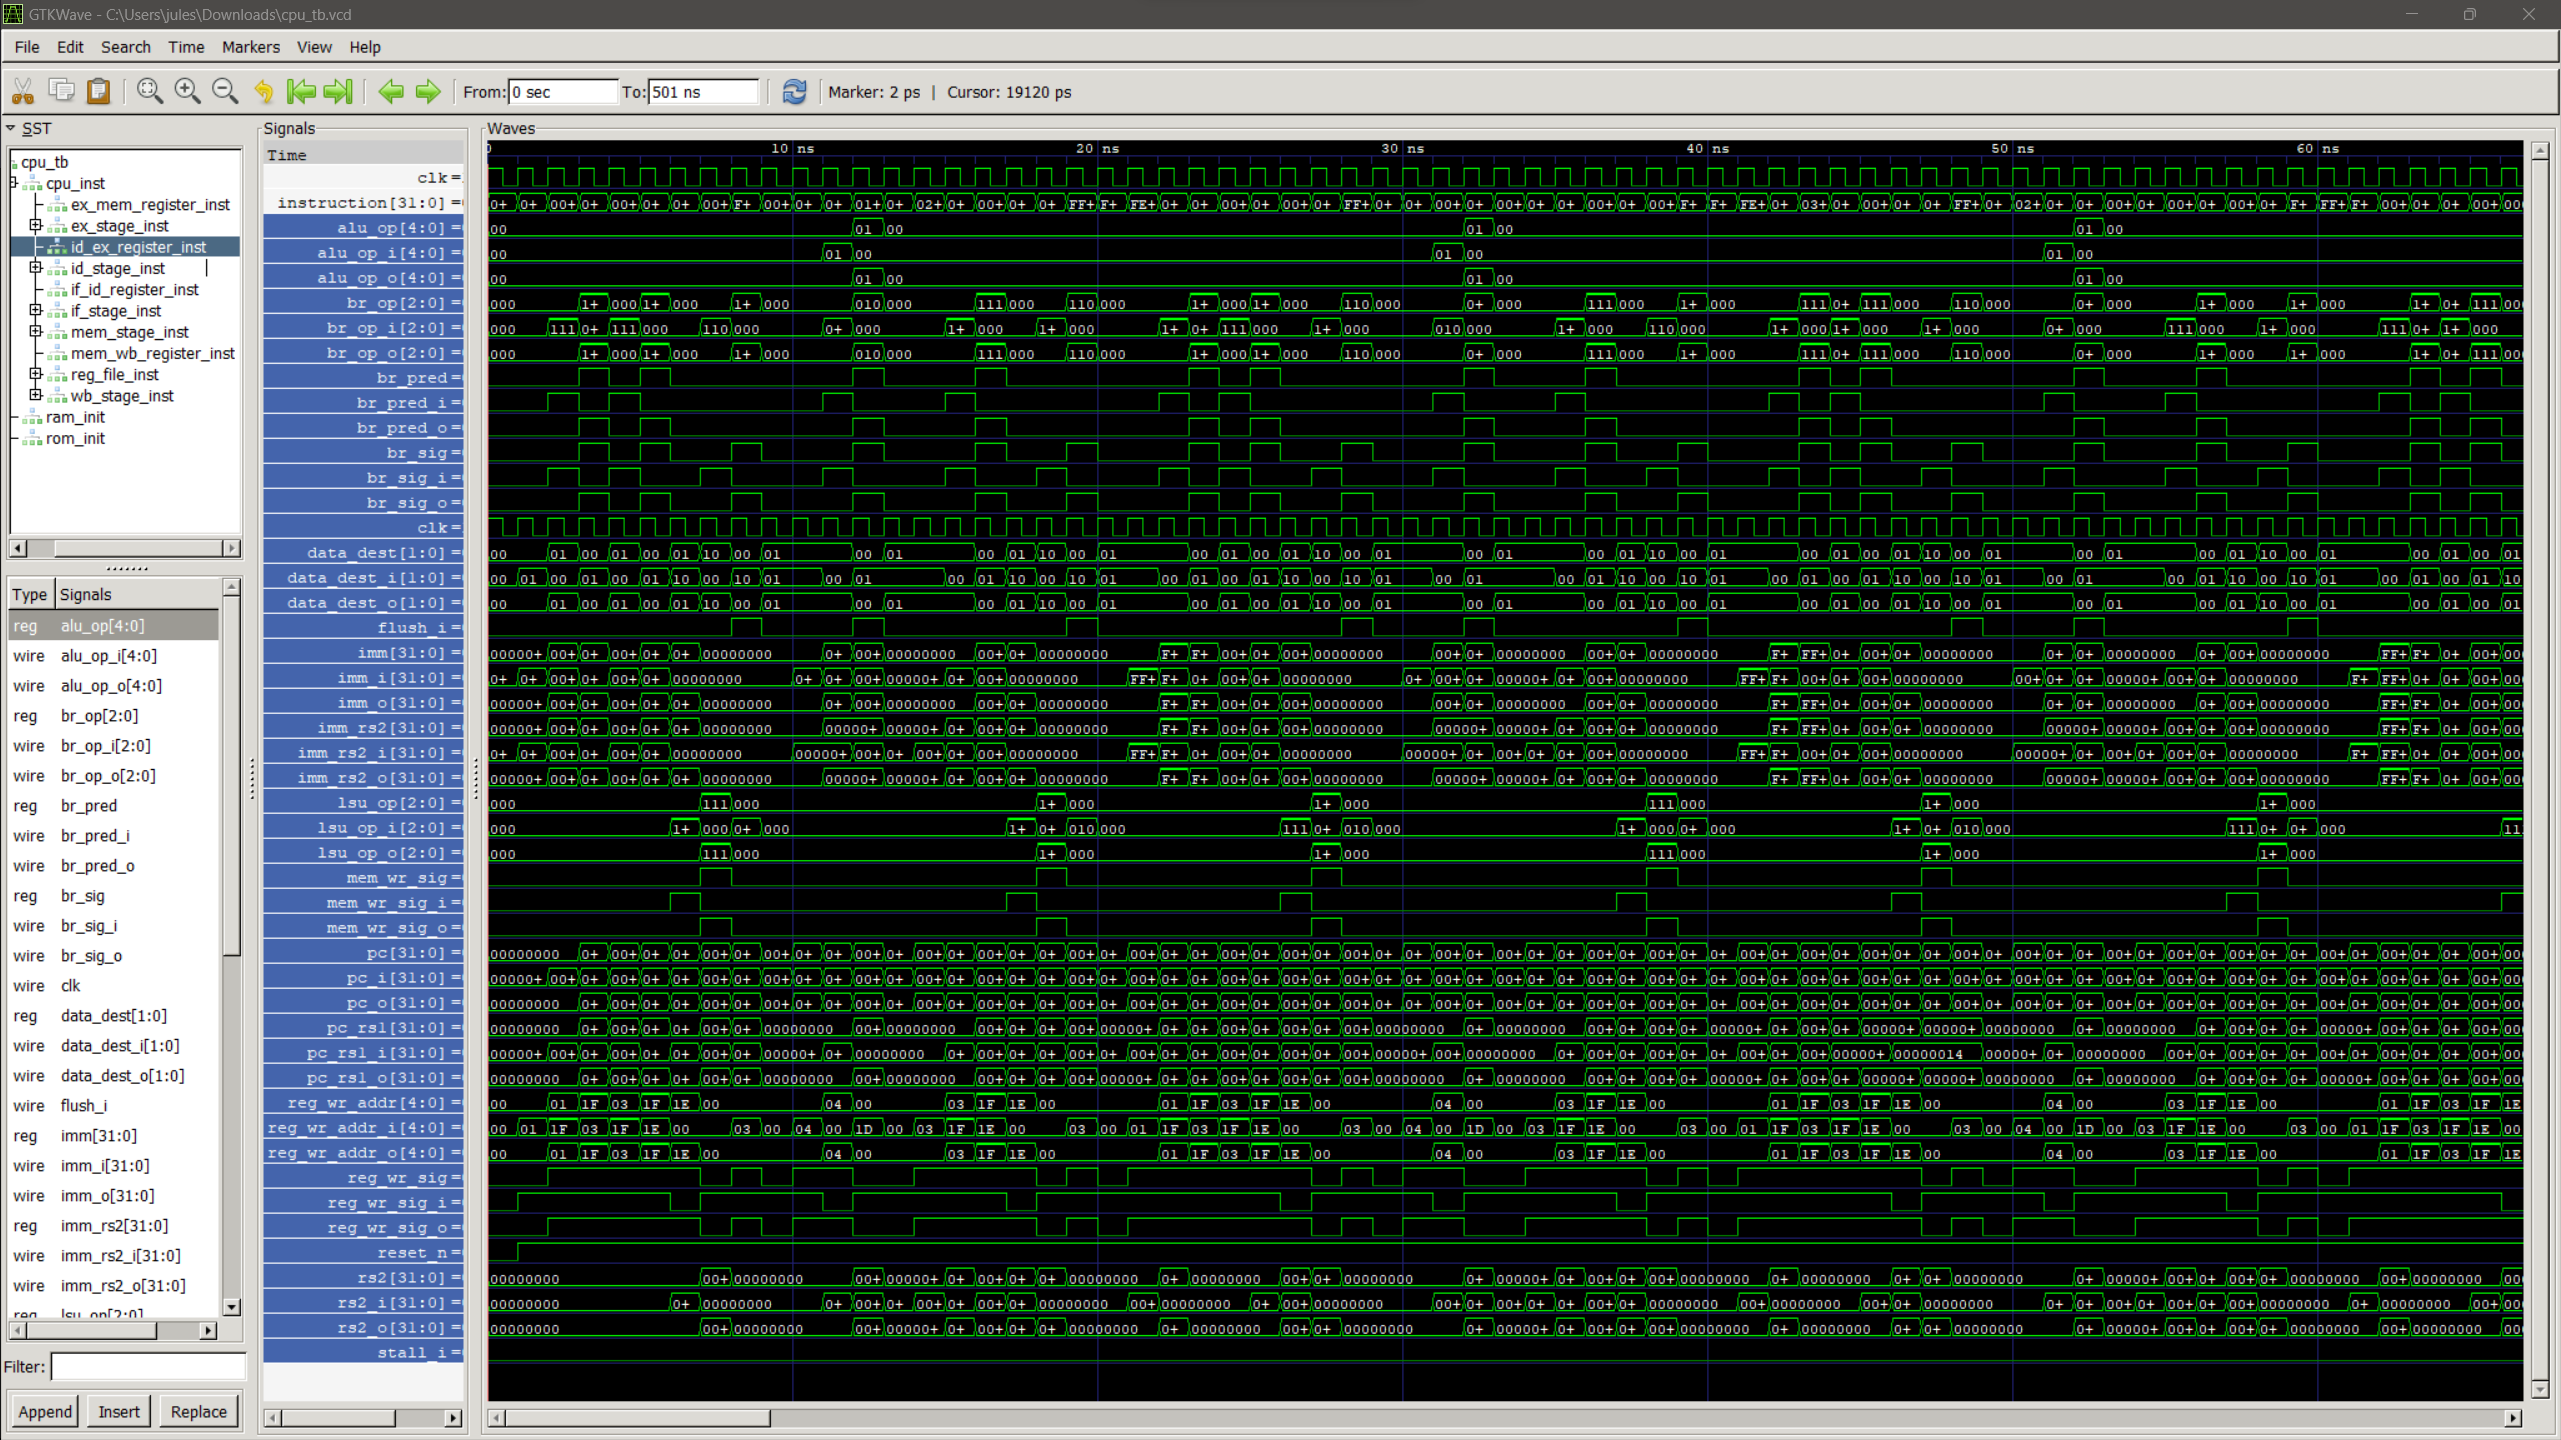
\includegraphics[width=1\textwidth]{testing/images/gtkwave.png}
    \caption{GTKWave output of the CPU testbench}
    \label{fig:gtkwave}
\end{figure}

